\documentclass{standalone}
\usepackage{tikz}
\usepackage{ctex,siunitx}
\setCJKmainfont{Noto Serif CJK SC}
\usepackage{tkz-euclide}
\usepackage{amsmath}
\usepackage{wasysym}
\usetikzlibrary{patterns, calc}
\usetikzlibrary {decorations.pathmorphing, decorations.pathreplacing, decorations.shapes,}
\begin{document}
\small
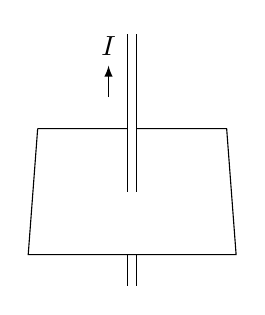
\begin{tikzpicture}[>=latex,xscale=0.6,yscale=0.4]
  \draw (-2,2)--(2,2)--(2.2, -2)--(-2.2,-2)--(-2,2);
  \fill[white](-.1,0) rectangle (.1,5);
  \draw (-0.1,0)--(-0.1,5); \draw (0.1,0)--(0.1,5);
  \draw (-0.1,-2)--(-0.1,-3);
  \draw (0.1,-2)--(0.1,-3);
  \draw[->] (-.5, 3)--(-.5,4)node[above]{$I$};
\end{tikzpicture}
\end{document}